\documentclass[12pt,a4paper]{article}

% === Packages ===
\usepackage[utf8]{inputenc}
\usepackage[romanian]{babel}
\usepackage[T1]{fontenc}
\usepackage{geometry}
\usepackage{graphicx}
\usepackage{amsmath,amsfonts,amssymb}
\usepackage{listings}
\usepackage{xcolor}
\usepackage{hyperref}
\usepackage{booktabs}
\usepackage{float}
\usepackage{tikz}
\usetikzlibrary{shapes,arrows,positioning}
\usepackage{fancyhdr}
\usepackage{titlesec}
\usepackage{tocloft}
\usepackage{enumitem}
\usepackage{caption}
\usepackage{array}
\usepackage{longtable}

% === Page Setup ===
\geometry{
    left=2.5cm,
    right=2.5cm,
    top=2.5cm,
    bottom=2.5cm
}

% === Header/Footer ===
\pagestyle{fancy}
\fancyhf{}
\fancyhead[L]{Proiect Criptografie}
\fancyhead[R]{Simulare One-Time Pad}
\fancyfoot[C]{\thepage}
\renewcommand{\headrulewidth}{0.4pt}
\renewcommand{\footrulewidth}{0.4pt}

% === Colors ===
\definecolor{codegreen}{rgb}{0,0.6,0}
\definecolor{codegray}{rgb}{0.5,0.5,0.5}
\definecolor{codepurple}{rgb}{0.58,0,0.82}
\definecolor{backcolour}{rgb}{0.95,0.95,0.92}
\definecolor{linkblue}{RGB}{0,0,180}

% === Hyperref Setup ===
\hypersetup{
    colorlinks=true,
    linkcolor=linkblue,
    filecolor=magenta,
    urlcolor=cyan,
    pdftitle={Proiect Criptografie - OTP},
    pdfauthor={Student},
}

% === Code Listings ===
\lstdefinestyle{gostyle}{
    backgroundcolor=\color{backcolour},
    commentstyle=\color{codegreen},
    keywordstyle=\color{magenta},
    numberstyle=\tiny\color{codegray},
    stringstyle=\color{codepurple},
    basicstyle=\ttfamily\footnotesize,
    breakatwhitespace=false,
    breaklines=true,
    captionpos=b,
    keepspaces=true,
    numbers=left,
    numbersep=5pt,
    showspaces=false,
    showstringspaces=false,
    showtabs=false,
    tabsize=2,
    frame=single
}
\lstset{style=gostyle}

% === Title Formatting ===
\titleformat{\section}
    {\normalfont\Large\bfseries}{\thesection}{1em}{}
\titleformat{\subsection}
    {\normalfont\large\bfseries}{\thesubsection}{1em}{}

% === Document Start ===
\begin{document}

% ============================================================
% 1. PRIMA PAGINĂ
% ============================================================
\begin{titlepage}
    \centering
    \vspace*{2cm}

    {\scshape\LARGE Universitatea \par}
    {\scshape\Large Facultatea de Informatică\par}

    \vspace{3cm}

    {\Huge\bfseries Proiect Criptografie\par}
    \vspace{0.5cm}
    {\LARGE\bfseries Simularea unui Mecanism\\One-Time Pad (OTP)\par}

    \vspace{4cm}

    \begin{minipage}{0.4\textwidth}
        \begin{flushleft}
            \textbf{Student:}\\
            Nume Prenume\\
            Grupa: XXX
        \end{flushleft}
    \end{minipage}
    \begin{minipage}{0.4\textwidth}
        \begin{flushright}
            \textbf{Profesor coordonator:}\\
            Prof. Dr. Nume Prenume\\
            Departamentul de Informatică
        \end{flushright}
    \end{minipage}

    \vfill

    {\large Data: \today\par}
    {\large Anul Universitar 2024-2025\par}
\end{titlepage}

% === Table of Contents ===
\tableofcontents
\newpage

% ============================================================
% 2. INTRODUCERE
% ============================================================
\section{Introducere}

\subsection{Contextul și Relevanța Temei}

Într-o eră digitală în care comunicațiile electronice sunt omniprezente, securitatea informației a devenit o necesitate fundamentală. Criptografia, știința transformării informației pentru a o proteja de accesul neautorizat, stă la baza securității în domenii precum:

\begin{itemize}
    \item Comunicații militare și diplomatice
    \item Tranzacții bancare și financiare
    \item Protecția datelor personale
    \item Comunicații private între indivizi
\end{itemize}

One-Time Pad (OTP) ocupă un loc special în istoria criptografiei, fiind \textbf{singurul sistem de criptare cu securitate perfectă demonstrată matematic}. Claude Shannon a demonstrat acest lucru în lucrarea sa fundamentală din 1949, "Communication Theory of Secrecy Systems".

\subsection{Scopul General al Proiectului}

Acest proiect își propune implementarea și demonstrarea practică a algoritmului One-Time Pad, evidențiind:
\begin{itemize}
    \item Principiile fundamentale ale criptării simetrice
    \item Operația XOR ca bază a criptării OTP
    \item Importanța generării securizate a cheilor criptografice
    \item Condițiile necesare pentru obținerea securității perfecte
\end{itemize}

\subsection{Aplicații Practice}

Deși OTP are limitări practice (problema distribuției cheilor), a fost utilizat istoric în:
\begin{itemize}
    \item \textbf{Linia roșie Moscova-Washington} - comunicație directă între liderii SUA și URSS în timpul Războiului Rece
    \item \textbf{Comunicații diplomatice} - transmiterea mesajelor clasificate între ambasade
    \item \textbf{Spionaj} - agenții foloseau blocuri de chei pentru mesaje scurte
\end{itemize}

În prezent, OTP servește ca bază teoretică pentru înțelegerea securității criptografice și este relevant în contextul criptografiei cuantice.

% ============================================================
% 3. OBIECTIVE
% ============================================================
\section{Obiective}

\subsection{Obiective Principale}

Proiectul își propune atingerea următoarelor obiective:

\begin{enumerate}
    \item \textbf{Implementarea algoritmului OTP} - Dezvoltarea unui sistem funcțional de criptare/decriptare bazat pe One-Time Pad

    \item \textbf{Generarea securizată a cheilor} - Utilizarea pachetului \texttt{crypto/rand} din Go pentru generarea cheilor criptografic securizate (CSPRNG)

    \item \textbf{Demonstrarea operației XOR} - Ilustrarea practică a modului în care XOR asigură criptarea și decriptarea

    \item \textbf{Afișarea în multiple formate} - Prezentarea mesajului original, cheii și mesajului criptat în format text, ASCII și hexazecimal

    \item \textbf{Verificarea corectitudinii} - Demonstrarea că decriptarea produce mesajul original

    \item \textbf{Salvarea rezultatelor} - Posibilitatea de export a cheii și mesajului criptat în fișiere
\end{enumerate}

\subsection{Rezultate Așteptate}

La finalizarea proiectului, se așteaptă:
\begin{itemize}
    \item O aplicație web funcțională cu interfață React și backend Go
    \item Demonstrarea practică a criptării OTP cu afișare în multiple formate
    \item Documentație completă a implementării
    \item Înțelegerea aprofundată a principiilor criptografice fundamentale
\end{itemize}

% ============================================================
% 4. FUNDAMENTE TEORETICE
% ============================================================
\section{Fundamente Teoretice}

\subsection{Principiile Algoritmului One-Time Pad}

One-Time Pad, inventat de Gilbert Vernam în 1917, funcționează prin combinarea fiecărui byte din mesaj cu byte-ul corespunzător din cheie folosind operația XOR.

\subsubsection{Formula Matematică}

\begin{equation}
    C_i = M_i \oplus K_i \quad \text{(Criptare)}
\end{equation}

\begin{equation}
    M_i = C_i \oplus K_i \quad \text{(Decriptare)}
\end{equation}

unde:
\begin{itemize}
    \item $C_i$ = byte-ul $i$ din ciphertext (mesajul criptat)
    \item $M_i$ = byte-ul $i$ din plaintext (mesajul original)
    \item $K_i$ = byte-ul $i$ din cheie
    \item $\oplus$ = operația XOR (sau exclusiv)
\end{itemize}

\subsection{Noțiuni Matematice - Operația XOR}

Operația XOR (sau exclusiv) este fundamentală pentru OTP:

\begin{table}[H]
\centering
\caption{Tabelul de adevăr pentru operația XOR}
\begin{tabular}{|c|c|c|}
\hline
\textbf{A} & \textbf{B} & \textbf{A $\oplus$ B} \\
\hline
0 & 0 & 0 \\
0 & 1 & 1 \\
1 & 0 & 1 \\
1 & 1 & 0 \\
\hline
\end{tabular}
\end{table}

\textbf{Proprietăți esențiale ale XOR:}
\begin{enumerate}
    \item \textbf{Comutativitate}: $A \oplus B = B \oplus A$
    \item \textbf{Asociativitate}: $(A \oplus B) \oplus C = A \oplus (B \oplus C)$
    \item \textbf{Element neutru}: $A \oplus 0 = A$
    \item \textbf{Auto-inversă}: $A \oplus A = 0$
    \item \textbf{Reversibilitate}: $(A \oplus B) \oplus B = A$
\end{enumerate}

Proprietatea de reversibilitate este esențială: aplicând XOR cu aceeași cheie, putem recupera mesajul original.

\subsection{Condiții pentru Securitate Perfectă}

Shannon a demonstrat că OTP oferă securitate perfectă dacă și numai dacă:

\begin{enumerate}
    \item \textbf{Aleatorietate completă}: Cheia trebuie generată folosind un CSPRNG (Cryptographically Secure Pseudo-Random Number Generator)
    \item \textbf{Lungime egală}: Cheia trebuie să aibă cel puțin lungimea mesajului
    \item \textbf{Utilizare unică}: Cheia nu trebuie folosită niciodată de două ori ("One-Time")
    \item \textbf{Secret}: Cheia trebuie păstrată secretă și distribuită în siguranță
\end{enumerate}

\subsection{Avantaje și Limitări}

\begin{table}[H]
\centering
\caption{Avantaje și limitări One-Time Pad}
\begin{tabular}{|p{7cm}|p{7cm}|}
\hline
\textbf{Avantaje} & \textbf{Limitări} \\
\hline
Securitate perfectă matematică & Cheia trebuie să fie la fel de lungă ca mesajul \\
\hline
Imposibil de spart (dacă respectă condițiile) & Problema distribuției securizate a cheilor \\
\hline
Algoritm simplu și rapid & Fiecare cheie se folosește o singură dată \\
\hline
Nu necesită putere de calcul mare & Impractică pentru volume mari de date \\
\hline
\end{tabular}
\end{table}

\subsection{Pericolul Reutilizării Cheii}

Reutilizarea cheii compromite complet securitatea OTP:

\begin{align}
    C_1 &= M_1 \oplus K \\
    C_2 &= M_2 \oplus K \\
    C_1 \oplus C_2 &= M_1 \oplus M_2
\end{align}

XOR-ul celor două ciphertexturi elimină cheia, permițând atacuri de crib dragging și analiză de frecvență.

\textbf{Exemplu istoric}: Proiectul VENONA al NSA a reușit să spargă mesaje sovietice tocmai datorită reutilizării cheilor OTP în anii 1940.

% ============================================================
% 5. METODOLOGIE ȘI IMPLEMENTARE
% ============================================================
\section{Metodologie și Implementare}

\subsection{Tehnologii Utilizate}

\begin{itemize}
    \item \textbf{Backend}: Go (Golang)
        \begin{itemize}
            \item \texttt{crypto/rand} - generare cheie criptografic securizată
            \item \texttt{encoding/json} - serializare/deserializare JSON
            \item \texttt{net/http} - server HTTP pentru API REST
        \end{itemize}
    \item \textbf{Frontend}: React 19 + Tailwind CSS
        \begin{itemize}
            \item Hooks (useState, useCallback) - state management
            \item Fetch API - comunicare cu backend
            \item Tailwind CSS - stilizare
        \end{itemize}
\end{itemize}

\subsection{Arhitectura Aplicației}

\begin{figure}[H]
\centering
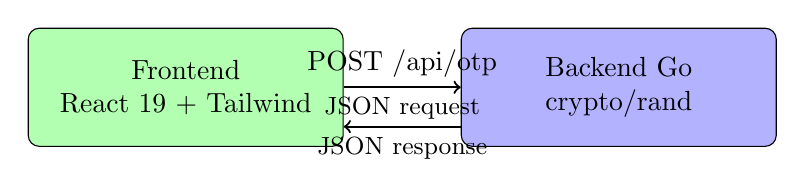
\begin{tikzpicture}[
    node distance=2.5cm,
    box/.style={draw, rectangle, rounded corners, minimum width=4cm, minimum height=1.5cm, align=center}
]
    \node[box, fill=green!30] (frontend) {Frontend\\React 19 + Tailwind};
    \node[box, fill=blue!30, right of=frontend, xshift=3cm] (backend) {Backend Go\\crypto/rand};

    \draw[->, thick] (frontend.east) -- node[above] {POST /api/otp} node[below] {\small JSON request} (backend.west);
    \draw[<-, thick] ([yshift=-5mm]frontend.east) -- node[below] {\small JSON response} ([yshift=-5mm]backend.west);
\end{tikzpicture}
\caption{Arhitectura client-server a aplicației}
\end{figure}

\subsection{Structura Proiectului}

\begin{verbatim}
OTP-Project/
├── backend/
│   └── main.go               # Server Go cu crypto/rand
├── frontend-react/
│   └── src/
│       ├── App.jsx           # Componenta principală
│       └── components/
│           └── OTPSimulator.jsx  # Interfață utilizator
├── docs/
│   ├── presentation/
│   │   └── presentation.tex  # Prezentare Beamer
│   └── report/
│       └── project_report.tex # Acest raport
└── README.md
\end{verbatim}

\subsection{Pașii de Implementare}

\subsubsection{Pasul 1: Primirea Mesajului}
Frontend-ul trimite mesajul text către backend printr-un request POST.

\subsubsection{Pasul 2: Generarea Cheii}
Backend-ul generează o cheie aleatorie de aceeași lungime cu mesajul folosind \texttt{crypto/rand}.

\subsubsection{Pasul 3: Criptarea}
Se aplică operația XOR între fiecare byte al mesajului și byte-ul corespunzător al cheii.

\subsubsection{Pasul 4: Decriptarea (Verificare)}
Se aplică din nou XOR între mesajul criptat și cheie pentru a verifica corectitudinea.

\subsubsection{Pasul 5: Returnarea Rezultatelor}
Backend-ul returnează toate datele în format JSON: mesaj original, cheie, criptat, decriptat (în formate text, ASCII, hex).

\subsection{Implementare Backend (Go)}

\begin{lstlisting}[language=Go, caption=Generarea cheii cu crypto/rand]
// genereaza cheie aleatorie securizata folosind crypto/rand
// asta e CSPRNG - cryptographically secure pseudo-random
func generateKey(length int) ([]byte, error) {
    key := make([]byte, length)
    _, err := rand.Read(key)  // crypto/rand.Read
    if err != nil {
        return nil, err
    }
    return key, nil
}
\end{lstlisting}

\begin{lstlisting}[language=Go, caption=Operația XOR pentru criptare/decriptare]
// xor intre doua array-uri de bytes
// aceeasi functie pentru criptare si decriptare
func xorBytes(a, b []byte) []byte {
    result := make([]byte, len(a))
    for i := 0; i < len(a); i++ {
        result[i] = a[i] ^ b[i]
    }
    return result
}
\end{lstlisting}

\begin{lstlisting}[language=Go, caption=Handler-ul principal OTP]
func handleOTP(w http.ResponseWriter, r *http.Request) {
    var req OTPRequest
    json.NewDecoder(r.Body).Decode(&req)

    // 1. convertim mesajul la bytes
    messageBytes := []byte(req.Message)

    // 2. generam cheie de aceeasi lungime
    keyBytes, _ := generateKey(len(messageBytes))

    // 3. criptam cu xor
    encryptedBytes := xorBytes(messageBytes, keyBytes)

    // 4. decriptam pentru verificare
    decryptedBytes := xorBytes(encryptedBytes, keyBytes)

    // 5. verificam ca decriptarea = original
    isMatch := string(decryptedBytes) == req.Message

    // 6. returnam rezultatele
    response := OTPResponse{
        OriginalText:  req.Message,
        OriginalHex:   bytesToHexSpaced(messageBytes),
        KeyHex:        bytesToHexSpaced(keyBytes),
        EncryptedHex:  bytesToHexSpaced(encryptedBytes),
        DecryptedText: string(decryptedBytes),
        IsMatch:       isMatch,
    }
    json.NewEncoder(w).Encode(response)
}
\end{lstlisting}

\subsection{Diagrama Fluxului de Criptare/Decriptare}

\begin{figure}[H]
\centering
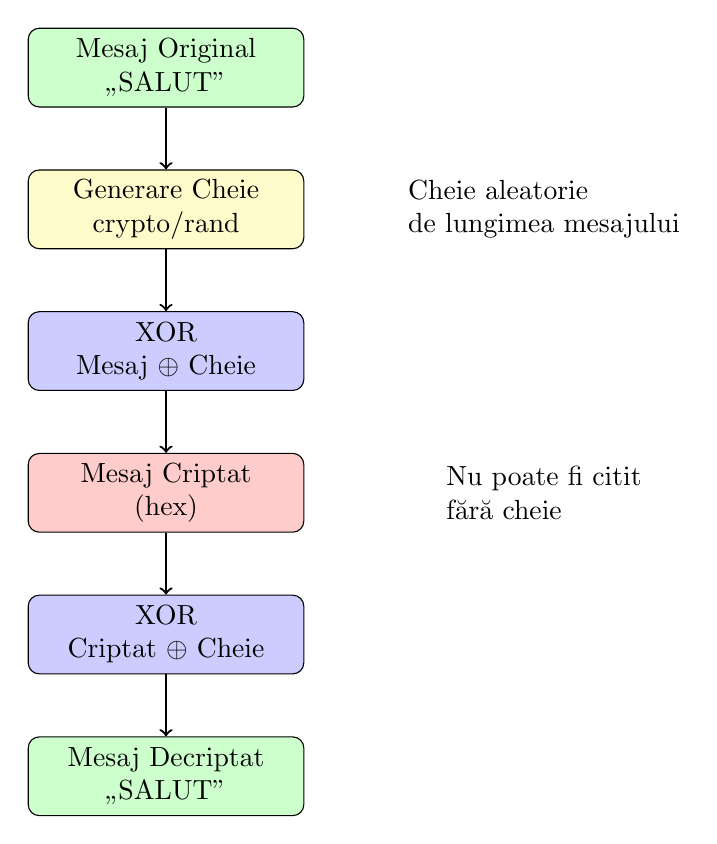
\begin{tikzpicture}[
    node distance=1.8cm,
    box/.style={draw, rectangle, rounded corners, minimum width=3.5cm, minimum height=1cm, align=center},
    arrow/.style={->, thick}
]
    \node[box, fill=green!20] (input) {Mesaj Original\\„SALUT"};
    \node[box, fill=yellow!20, below of=input] (keygen) {Generare Cheie\\crypto/rand};
    \node[box, fill=blue!20, below of=keygen] (xor1) {XOR\\Mesaj $\oplus$ Cheie};
    \node[box, fill=red!20, below of=xor1] (encrypted) {Mesaj Criptat\\(hex)};
    \node[box, fill=blue!20, below of=encrypted] (xor2) {XOR\\Criptat $\oplus$ Cheie};
    \node[box, fill=green!20, below of=xor2] (output) {Mesaj Decriptat\\„SALUT"};

    \draw[arrow] (input) -- (keygen);
    \draw[arrow] (keygen) -- (xor1);
    \draw[arrow] (xor1) -- (encrypted);
    \draw[arrow] (encrypted) -- (xor2);
    \draw[arrow] (xor2) -- (output);

    \node[right of=keygen, xshift=3cm, align=left] {Cheie aleatorie\\de lungimea mesajului};
    \node[right of=encrypted, xshift=3cm, align=left] {Nu poate fi citit\\fără cheie};
\end{tikzpicture}
\caption{Fluxul de criptare și decriptare OTP}
\end{figure}

% ============================================================
% 6. REZULTATE ȘI TESTARE
% ============================================================
\section{Rezultate și Testare}

\subsection{Exemple de Rulare}

\subsubsection{Exemplul 1: Mesaj simplu „ABC"}

\begin{table}[H]
\centering
\caption{Rezultatul criptării pentru mesajul „ABC"}
\begin{tabular}{|l|l|}
\hline
\textbf{Câmp} & \textbf{Valoare} \\
\hline
Mesaj original (text) & ABC \\
\hline
Mesaj original (ASCII) & 65 66 67 \\
\hline
Mesaj original (hex) & 41 42 43 \\
\hline
Cheie OTP (hex) & A7 3F 82 \\
\hline
Mesaj criptat (hex) & E6 7D C1 \\
\hline
Mesaj decriptat (text) & ABC \\
\hline
Verificare & ✓ Identic cu originalul \\
\hline
\end{tabular}
\end{table}

\subsubsection{Exemplul 2: Mesaj românesc „SALUT"}

\begin{table}[H]
\centering
\caption{Rezultatul criptării pentru mesajul „SALUT"}
\begin{tabular}{|l|l|}
\hline
\textbf{Câmp} & \textbf{Valoare} \\
\hline
Mesaj original (text) & SALUT \\
\hline
Mesaj original (ASCII) & 83 65 76 85 84 \\
\hline
Mesaj original (hex) & 53 41 4C 55 54 \\
\hline
Cheie OTP (hex) & B2 7E 9A 3D F1 \\
\hline
Mesaj criptat (hex) & E1 3F D6 68 A5 \\
\hline
Mesaj decriptat (text) & SALUT \\
\hline
Verificare & ✓ Identic cu originalul \\
\hline
\end{tabular}
\end{table}

\subsection{Analiza Performanței}

\begin{table}[H]
\centering
\caption{Timpi de execuție pentru diferite lungimi de mesaj}
\begin{tabular}{|c|c|c|}
\hline
\textbf{Lungime mesaj} & \textbf{Timp generare cheie} & \textbf{Timp criptare XOR} \\
\hline
10 bytes & < 1 ms & < 1 ms \\
\hline
100 bytes & < 1 ms & < 1 ms \\
\hline
1 KB & < 1 ms & < 1 ms \\
\hline
10 KB & 1-2 ms & < 1 ms \\
\hline
\end{tabular}
\end{table}

Operația XOR este extrem de rapidă, complexitatea fiind $O(n)$ unde $n$ este lungimea mesajului.

\subsection{Analiza Corectitudinii}

Sistemul verifică automat că:
\begin{enumerate}
    \item Cheia generată are exact lungimea mesajului
    \item Decriptarea produce exact mesajul original
    \item Fiecare rulare generează o cheie diferită (aleatorietate)
\end{enumerate}

\subsection{Analiza Securității}

\textbf{Puncte forte ale implementării:}
\begin{itemize}
    \item Folosirea \texttt{crypto/rand} din Go care este un CSPRNG
    \item Cheia este generată pe server, nu în browser
    \item Lungimea cheii egalează întotdeauna lungimea mesajului
\end{itemize}

\textbf{Limitări (pentru utilizare în producție):}
\begin{itemize}
    \item Nu există mecanism de distribuție securizată a cheilor
    \item Cheile nu sunt stocate permanent (generat la fiecare request)
    \item Comunicația client-server ar trebui să fie prin HTTPS
\end{itemize}

% ============================================================
% 7. CONCLUZII
% ============================================================
\section{Concluzii}

\subsection{Obiective Atinse}

Toate obiectivele propuse au fost atinse:

\begin{enumerate}
    \item ✓ \textbf{Implementare OTP funcțională} - Aplicația criptează și decriptează corect
    \item ✓ \textbf{Generare securizată chei} - Folosind \texttt{crypto/rand} din Go
    \item ✓ \textbf{Demonstrare XOR} - Vizibilă în cod și rezultate
    \item ✓ \textbf{Multiple formate} - Text, ASCII, hexazecimal
    \item ✓ \textbf{Verificare automată} - Confirmarea decriptării corecte
    \item ✓ \textbf{Export fișiere} - Salvare cheie și mesaj criptat
\end{enumerate}

\subsection{Ce s-a Învățat}

Prin implementarea acestui proiect am aprofundat:

\begin{enumerate}
    \item \textbf{Securitatea perfectă există} - OTP demonstrează că este posibilă matematic, dar vine cu costuri practice semnificative

    \item \textbf{Generarea cheilor este critică} - Diferența dintre \texttt{math/rand} (nesecurizat) și \texttt{crypto/rand} (CSPRNG) poate compromite complet securitatea

    \item \textbf{Simplitatea nu înseamnă slăbiciune} - XOR este o operație simplă dar fundamentală în criptografie

    \item \textbf{Disciplina utilizării} - „One-Time" înseamnă exact o singură utilizare a cheii

    \item \textbf{Arhitectura client-server} - Operațiile criptografice trebuie făcute pe server, nu în browser
\end{enumerate}

\subsection{Posibile Îmbunătățiri}

Pentru versiuni viitoare, se pot adăuga:

\begin{enumerate}
    \item \textbf{Distribuție cheie} - Implementarea unui canal securizat pentru partajarea cheilor
    \item \textbf{Stocare cheie} - Bază de date securizată pentru cheile generate
    \item \textbf{HTTPS} - Criptarea comunicației client-server
    \item \textbf{Interfață extinsă} - Suport pentru fișiere binare, nu doar text
    \item \textbf{Audit de securitate} - Analiză detaliată a potențialelor vulnerabilități
    \item \textbf{Comparație algoritmi} - Demonstrarea diferențelor față de AES, ChaCha20
\end{enumerate}

% ============================================================
% 8. BIBLIOGRAFIE
% ============================================================
\section*{Bibliografie}
\addcontentsline{toc}{section}{Bibliografie}

\subsection*{Suport Didactic}
\begin{enumerate}
    \item Materiale de curs Criptografie - Facultatea de Informatică
    \item Laboratoare practice de criptografie
\end{enumerate}

\subsection*{Cărți și Articole de Specialitate}
\begin{enumerate}
    \item Shannon, C. E. (1949). "Communication Theory of Secrecy Systems". Bell System Technical Journal, 28(4), 656-715.
    \item Stallings, W. (2017). "Cryptography and Network Security: Principles and Practice" (7th Edition). Pearson.
    \item Schneier, B. (2015). "Applied Cryptography: Protocols, Algorithms and Source Code in C" (20th Anniversary Edition). Wiley.
    \item Menezes, A. J., van Oorschot, P. C., Vanstone, S. A. (1996). "Handbook of Applied Cryptography". CRC Press.
\end{enumerate}

\subsection*{Documentația Bibliotecilor Utilizate}
\begin{enumerate}
    \item Go crypto/rand package - \url{https://pkg.go.dev/crypto/rand}
    \item Go encoding/json package - \url{https://pkg.go.dev/encoding/json}
    \item Go net/http package - \url{https://pkg.go.dev/net/http}
    \item React 19 Documentation - \url{https://react.dev/}
    \item Tailwind CSS Documentation - \url{https://tailwindcss.com/docs}
\end{enumerate}

\end{document}
